%!TEX root = ../Hardtung_PP_WiSe1920.tex

\section{Problems \& other Findings}
\label{sec:problems}

This section discusses decisions and problems during the development process.\\
Rendering the lines of the paper, all the arrows and other symbols could be done in a plethora of ways. Although the use of graphics libraries like JavaFx, libgdx, lwjgl or jogl was one of the options, the Origrammer relies only on Graphics2D. The more sophisticated graphics libraries were mostly developed for game development and offer a lot of features that were not necessary for this project. Using only the general shapes of Graphics2D removes a lot of unnecessary complexity while offering a similar outcome.
\\
To sum up, the Model Panel now consists of a JPanel on which a Graphics2D object is used to draw the diagram elements. But this decision also brought some restrictions and problems.


\subsection{Displaying of Arrows/Symbols}
\label{sec:displaySymbols}
As some arrows and symbols are quite complex it would have been preferable just to use images of the arrows/symbols instead of creating them with simple Shape objects. So the requirements were to display images with variable position, size and rotation. The most obvious solution was to place a JLabel for each arrow or symbol and use its \texttt{setIcon(BufferedImage img)} method to render a \texttt{BufferedImage img} of the arrows/symbols. Placing a JLabel on absolute x,y coordinates is done by using the \texttt{setBounds(x, y, width, height)} method with the mouse cursor \texttt{x} and \texttt{y} coordinates and the picture \texttt{width} and \texttt{height}. Unfortunately there didn't seem to be a way to rotate a JLabel itself, so another way had to be found. The next idea was to rotate the BufferedImage itself and that did work quite well after calculating the new bounds of the JLabel based on the BufferedImage size.\\
While that solution did technically work, the outcome was not satisfactory as the image quality suffered a lot when scaling and zooming. Using vector graphics instead of .png files would avoid this quality loss, but natively there was no way to load a .svg file into the \texttt{Image} or \texttt{BufferedImage} class. To solve this problem the library Batik\footnote{\url{https://xmlgraphics.apache.org/batik//}} was used. This allowed to load vector graphics of all arrows and symbols. Then after scaling and rotating, the vector graphics can be rasterized (again, with Batik) in order to use them as ImageIcons of the previously mentioned labels. Unfortunately rotating the arrows and symbols turned out to be a problem now. As .svg files contain no explicit width or height values, calculating the updated bounds of the label after a rotation was not longer possible. As a result the rotated BufferedImage got cut off at the old bounds of its label. That is why the current implementation uses a unique vector graphic for every 22.5° rotation and loads them when necessary. The 22.5° angle was deliberately chosen as the paper in origami often gets folded at 90°, 45° or 22.5° angles (smaller and smaller bisectors with 22.5° as the smallest angle commonly used).\\%source??????
\\
As a result the current implementation of using arrows and symbols works like this:

\begin{enumerate}[label=\textbf{\arabic*}.]
	\item Load the .svg file of an arrow or symbol with the required rotation
	\item Scale it as necessary
	\item Rasterize it with Batik to a BufferedImage
	\item Use this BufferedImage as an ImageIcon of a JLabel
	\item Place this JLabel with \texttt{label.setBounds(x, y, width, height)}  on the diagram (\texttt{width} and \texttt{height} are automatically determined by Batik when rasterizing).
\end{enumerate}
This solution fulfills almost all requirements, as arrows and symbols can be placed freely by absolute coordinates and they can be rotated and scaled without quality loss. But there are still two problems.\\
Firstly, the bounding box of the JLabel is always square and therefore not accurate. This is another problem with the missing width and height values of .svg files. Though this could potentially be fixed by individually calculating the new x and y coordinates as well as the new width and height after scaling and rotating an arrow or symbol.\\
The second problem is unwanted scaling when rotating an arrow or symbol. This happens when a long image is rotated to 45°, 135°, 225° or 315° (so the image goes from one corner to another) as the JLabel tries to display the largest ImageIcon possible within its bounds. Again, both of these problems can be traced back to the missing width and height values of vector graphics.\\
The most flexible and accurate solution that solves every problem would still be either to rebuild all arrows and symbols by hand with the simple Shape objects inside Java or to transcode vector graphics into the Shapes. These two approaches could be used in the future but couldn't be tested yet as both solutions would take a considerable amount of time and rewriting of existing code.

\subsection{Breaking Calculations}
\label{sec:breakingCalc}
One problem in the current version of Origrammer is a possibly wrong user input. In case of the \emph{Equal Angle} symbol the user has to specify 3 vertices on the diagram in a specific order. The first selected vertex is always the corner point (blue vertex on Fig. \ref{fig:equalAngle1}), the second vertex has to lie vertically (the red vertex) and the last one has to lie horizontally (green vertex) towards the corner point. When using this order, the resulting symbol is drawn correctly for all four quadrants of a coordinate plane. Consequently the \emph{Equal Angle} symbol can be drawn facing the top left, top right, bottom left or bottom right while also providing settings for a custom amount of dividers.
\begin{figure*}[h]
    \centering
    \begin{subfigure}[b]{0.4\textwidth}
        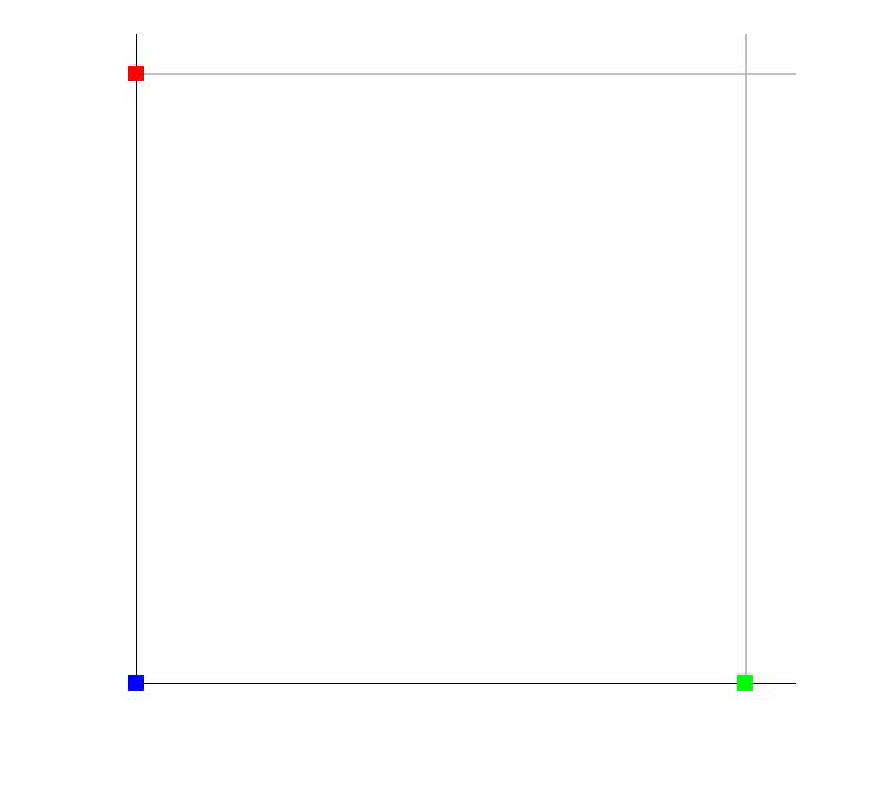
\includegraphics[width=\textwidth]{equalAngle1}
        \caption{Input}
        \label{fig:equalAngle1}
    \end{subfigure}
    \begin{subfigure}[b]{0.4\textwidth}
        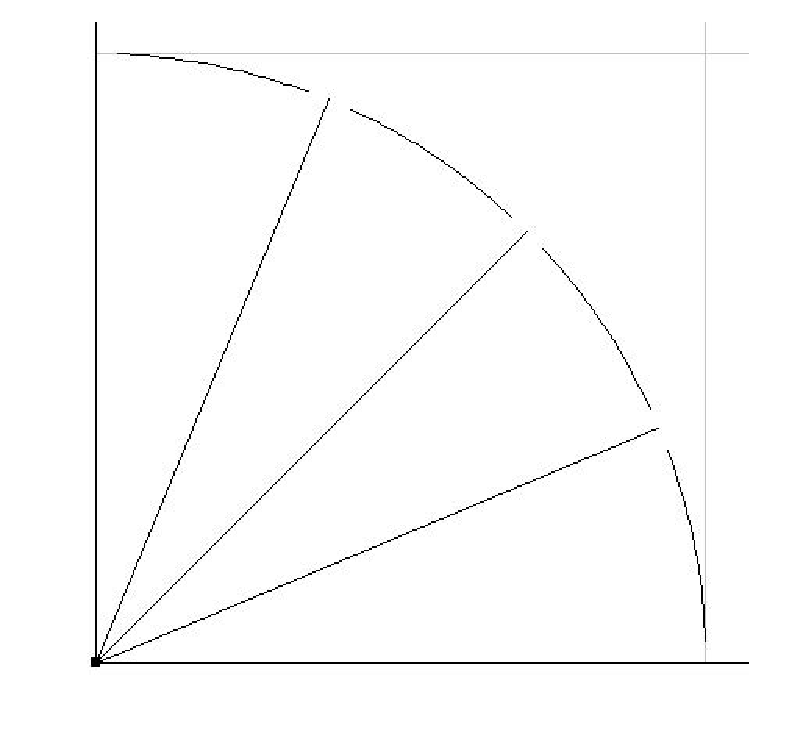
\includegraphics[width=\textwidth]{equalAngle2}
        \caption{Result}
        \label{fig:equalAngle2}
    \end{subfigure}
    \caption{Equal Angle Symbol}
\end{figure*}\\
This reliance on correct user input could be reduced with a tooltip or small explaining text when selecting the input mode or by implementing a detailed input validation for each symbol. Though the focus while developing the Origrammer was set on increasing functionality over usability first. This approach allowed a quicker implementation of all required features in order to demonstrate how a finished diagramming program could look like.


\subsection{Saving and Opening Files}

Being able to save and open diagrams created with the Origrammer was imperative to the usefulness of the program. A saved Origrammer file had to contain all relevant model information like the title, author, comments, recommended paper size, paper shape, paper color as well as the diagram information itself. Every line, arrow, symbol and the textual instructions for each step had to be included and correctly displayed after opening a file.


\subsection{Crossing Lines}

When inputting several overlapping lines, they should be split up and a new addressable vertex at their crossing points has to be created. Implementing this feature by itself was done relatively quickly. However, with the addition of the endpoint offsets for existing creases (see Section \ref{sec:generalRules} \emph{Creases should not contact the edges}) more variables had to be kept in mind. As the user can freely draw lines in different directions and in random order, a lot of edge cases had to be considered (see Fig. \ref{fig:crossingLines}). In the Origrammer, a basic line is represented, amongst other things,  by two points and two boolean values in case the lines should be drawn with an offset (for the previously mentioned existing creases).\\
\\
\texttt{OriLine(p0(x,y), p1(x,y), boolean startOffset, boolean endOffset);}
\begin{figure}[h]
	\centering
	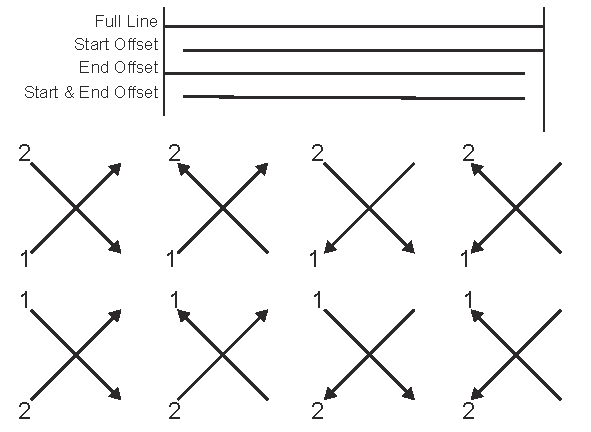
\includegraphics[width=0.6\textwidth]{CrossingLines}
	\caption{Crossing Lines Input Possibilities}
	\label{fig:crossingLines}
\end{figure}\\
So once two lines intersect each other, they have to be split up into four shorter lines. In order to accomplish this their \texttt{crossingPoint} is calculated and the new lines are created (see Fig. \ref{fig:crossingLinesExample}). Important here is, that the endpoint that contains the crossingPoint can not have an offset. This is also the point where the previously shown variety of different user inputs has to be taken into consideration. The start- and endpoints of a line change depending on what direction the user inputs them. Consequently a test had to be implemented that checks which direction a line in question is facing and that adjusts following calculations accordingly. Otherwise the offsets would be either drawn in the wrong order or too many offsets in general would be drawn. Additional complexity arises once an input line crosses multiple existing lines. In this case the input line has to be split into multiple smaller lines - at each crossing point of another existing line.

\begin{figure}[h]
	\centering
	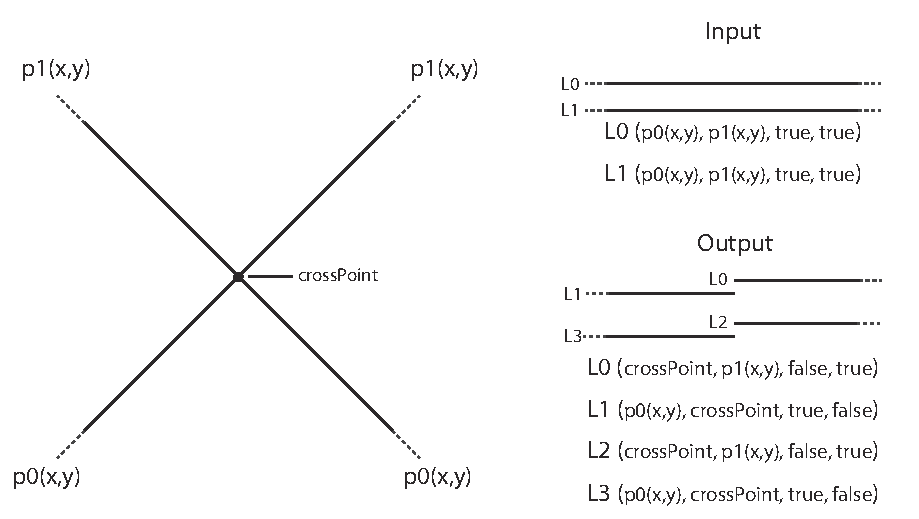
\includegraphics[width=0.9\textwidth]{CrossingLinesExample}
	\caption{Crossing Lines Example}
	\label{fig:crossingLinesExample}
\end{figure}

						
